%____________________________________________________________________________||
%FIXME: undefined reference to new systematic section
\section{Procedure for corrections to cross section for SM samples with 2015 data}
\label{app:sideband-corrections-old}

\subsection{Correction to the \gj sample}
\label{sec:sideband_corrections_gjets}
The situation is somehow different for \gj with respect to the other processes. 
In fact the cross section for this process is known only at LO and no $k$-factor is available. 
As a result, some disagreement between data and MC is expected in the single photon control region.
The observation confirms indeed this hypothesis, with the simulation underestimating the yields by $\sim 20\%$. \\
A correction is derived using a sideband in data, by inverting the \alphat cut. 
For $\scalht < 400$ GeV, events are selected in the interval $0.50 < \alphat < 0.52$, 
while for $\scalht \geq 400$ GeV the sideband is defined by the cut $0.50 < \alphat < 0.53$.
The data yields are corrected for the small QCD contamination (taken from MC) and divided by the expected number of events in the simulation. 

The correction factor to be applied to the GJets sample found with this procedure is $1.25 \pm 0.05$ (statistical error only). 
Cross-checks have been performed using other sidebands, obtained by inverting the \scalht and the \mhtmet cuts 
and have shown to give compatible results within the statistical precision. 
The sideband is shown in Fig.~\ref{fig:gjets_alphaTsideband}. 

\begin{figure}[!h]
  \centering
  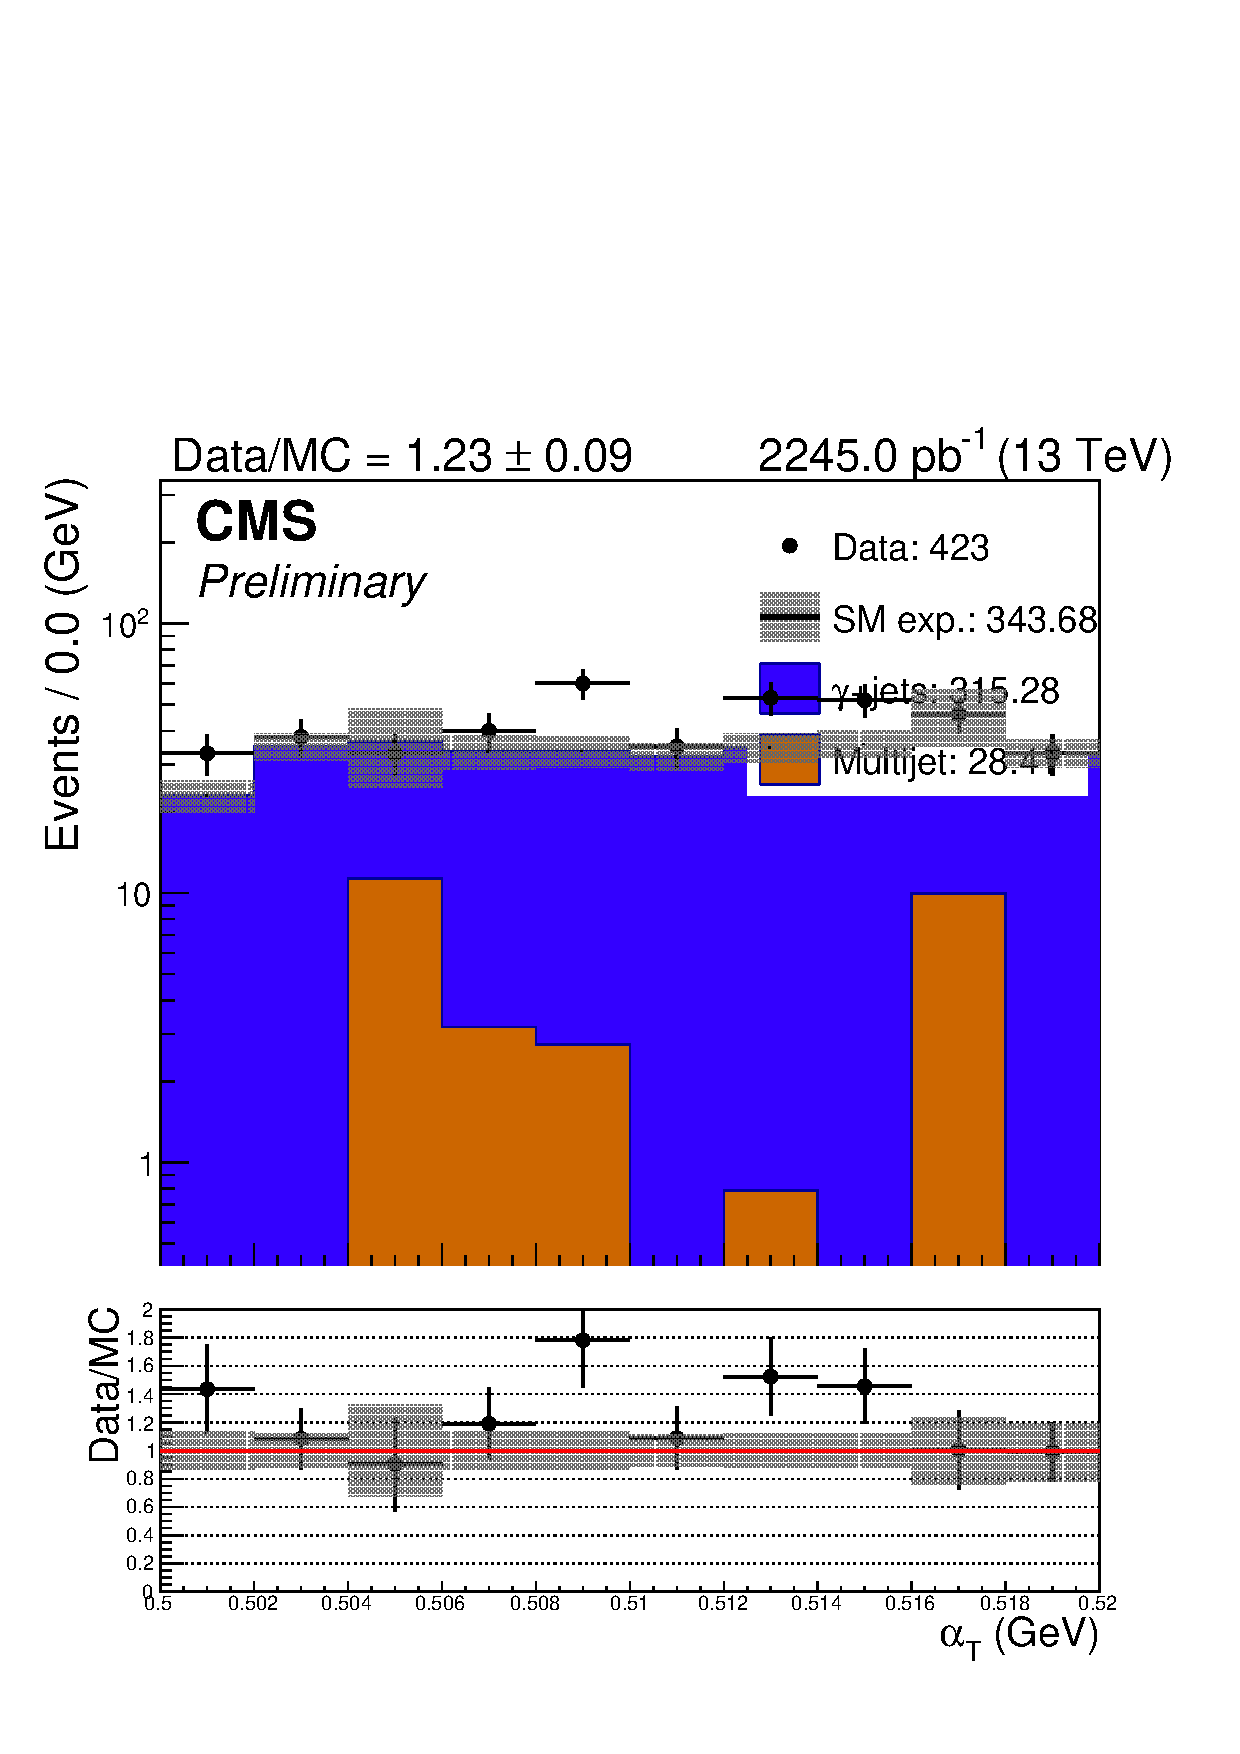
\includegraphics[width=0.45\textwidth]{figures/sidebandCorr/alphaTSideband_NMinusOne_AlphaT_GJets}
  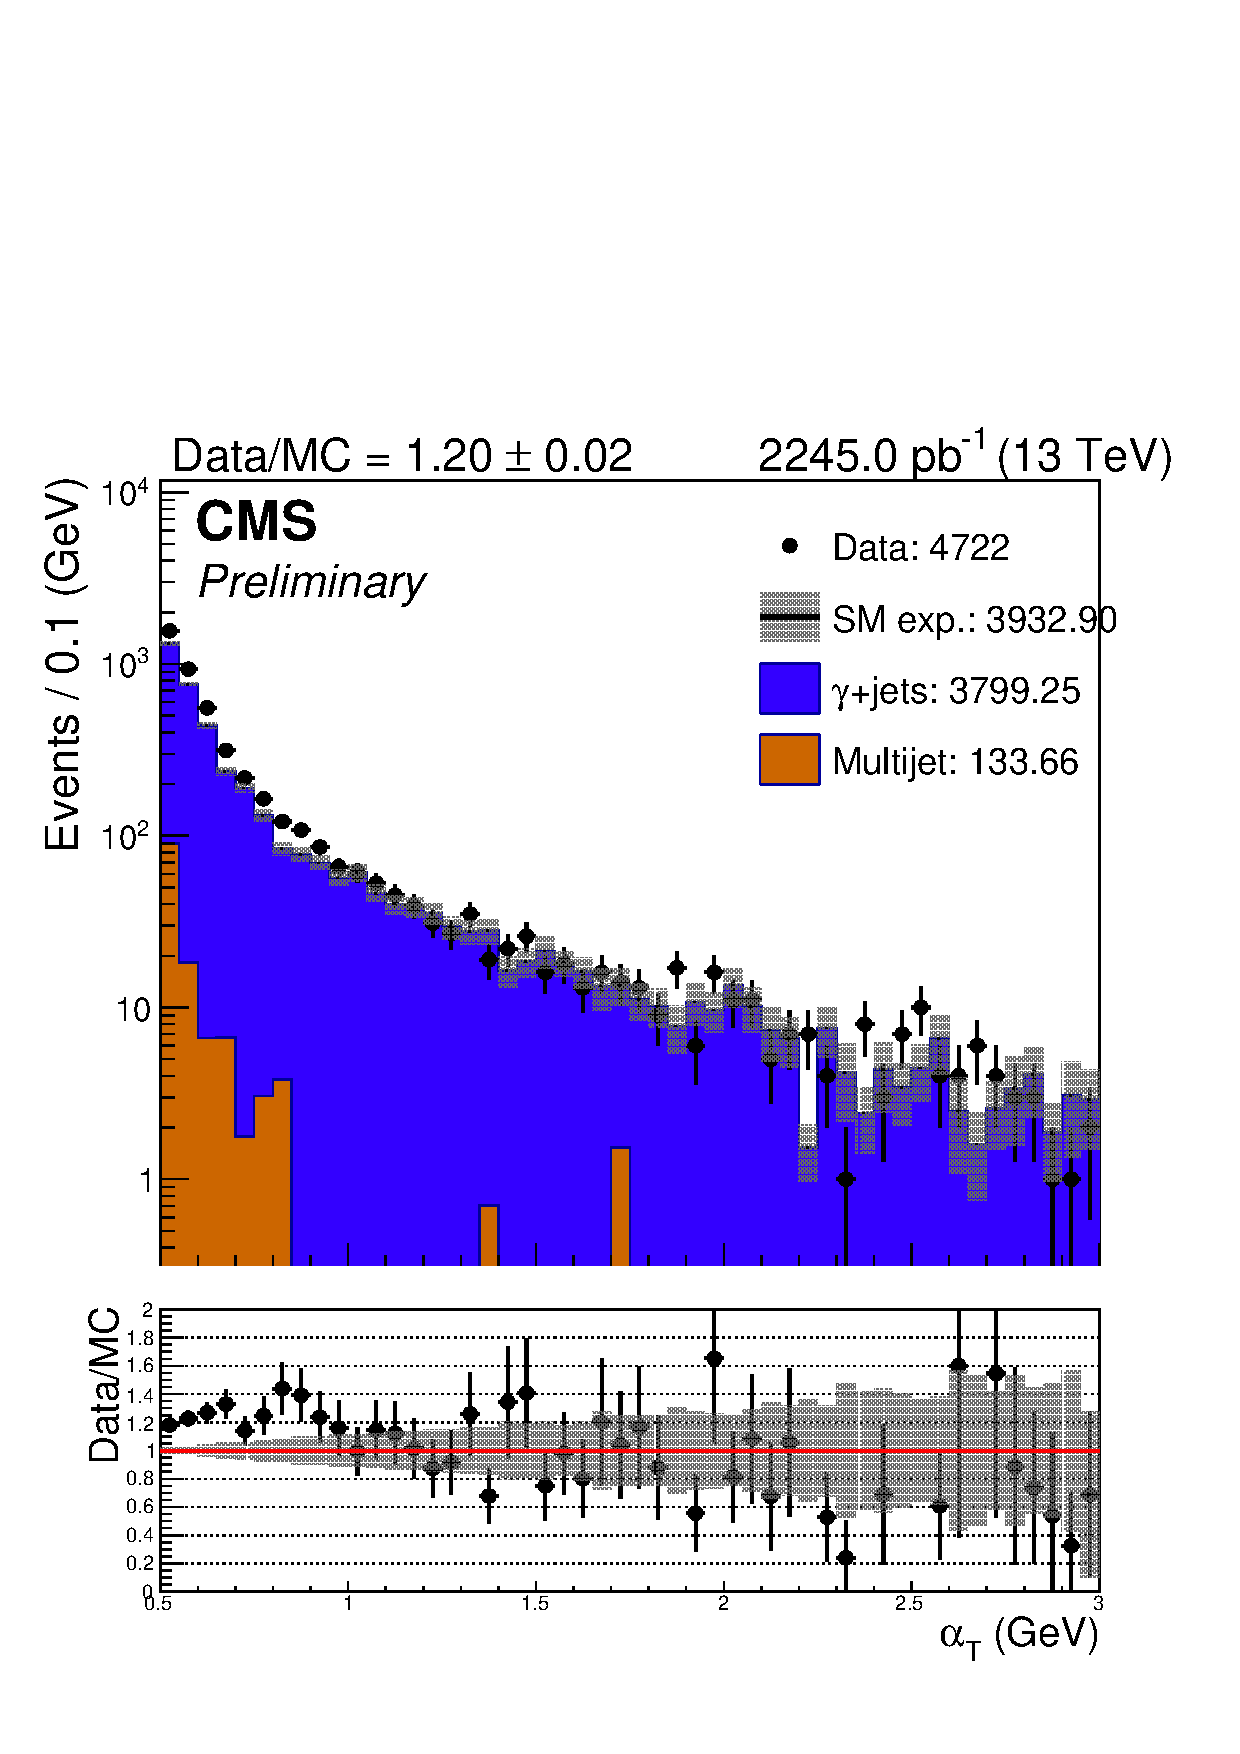
\includegraphics[width=0.45\textwidth]{figures/sidebandCorr/alphaT_NMinusOne_AlphaT_GJets}
  \caption{The \alphat distribution in the \gj control region in data compared with MC expectations. 
     The \alphat sideband used to derive the correction for the \gj process is shown on the left plot, while the full range is shown on the right.}
  \label{fig:gjets_alphaTsideband}
\end{figure}



\subsection{Correction to the $W$+jets, \ttbar+jets and $Z$+jets samples}
\label{sec:sideband_corrections_w_z_tt}
For the $W$+jets, \ttbar+jets and $Z$+jets samples the cross section is know with better accuracy with respect to the \gj process, 
with NLO QCD or better precision.
However, some inconsinstency could arise from the different cross section calculations, since for \wj and \zj the LO cross sections 
are corrected with NLO k-factor (1.21 and 1.23 respectively) while for \ttbar the full NNLO calculation is used. \\
The corrections for these processes are derived using a sideband defined by inverting the \mht cut, namely 
applying the selection $100 < \mht < 130$ GeV. 
Results are cross-checked using the $\mhtmet > 1.25$ sideband and found to give compatible results, within the statistical uncertainties. \\
In order to enrich the sidebands in each process, the following selection is applied for each sample:
\begin{itemize}
\item \wj: \mj, $\nj \leq 3$, $\nb = 0$
\item \zj: \mmj, $\nb = 0$
\item \ttj: \mj, $\nj \geq 2$, $\nb \geq 2$
\end{itemize}
These selections give a purity of 84\%, 93\% and 87\% respectively for \wj, \zj and \ttj. All contaminations are estimated from MC.

The corrections for the three processes are summarised in Tab.~\ref{tab:sbCorrs}.
The \mht distributions for these three selection are shown in Fig.~\ref{fig:wjets_MHTsideband}-\ref{fig:ttjets_MHTsideband}. \\

\begin{figure}[!h]
  \centering
  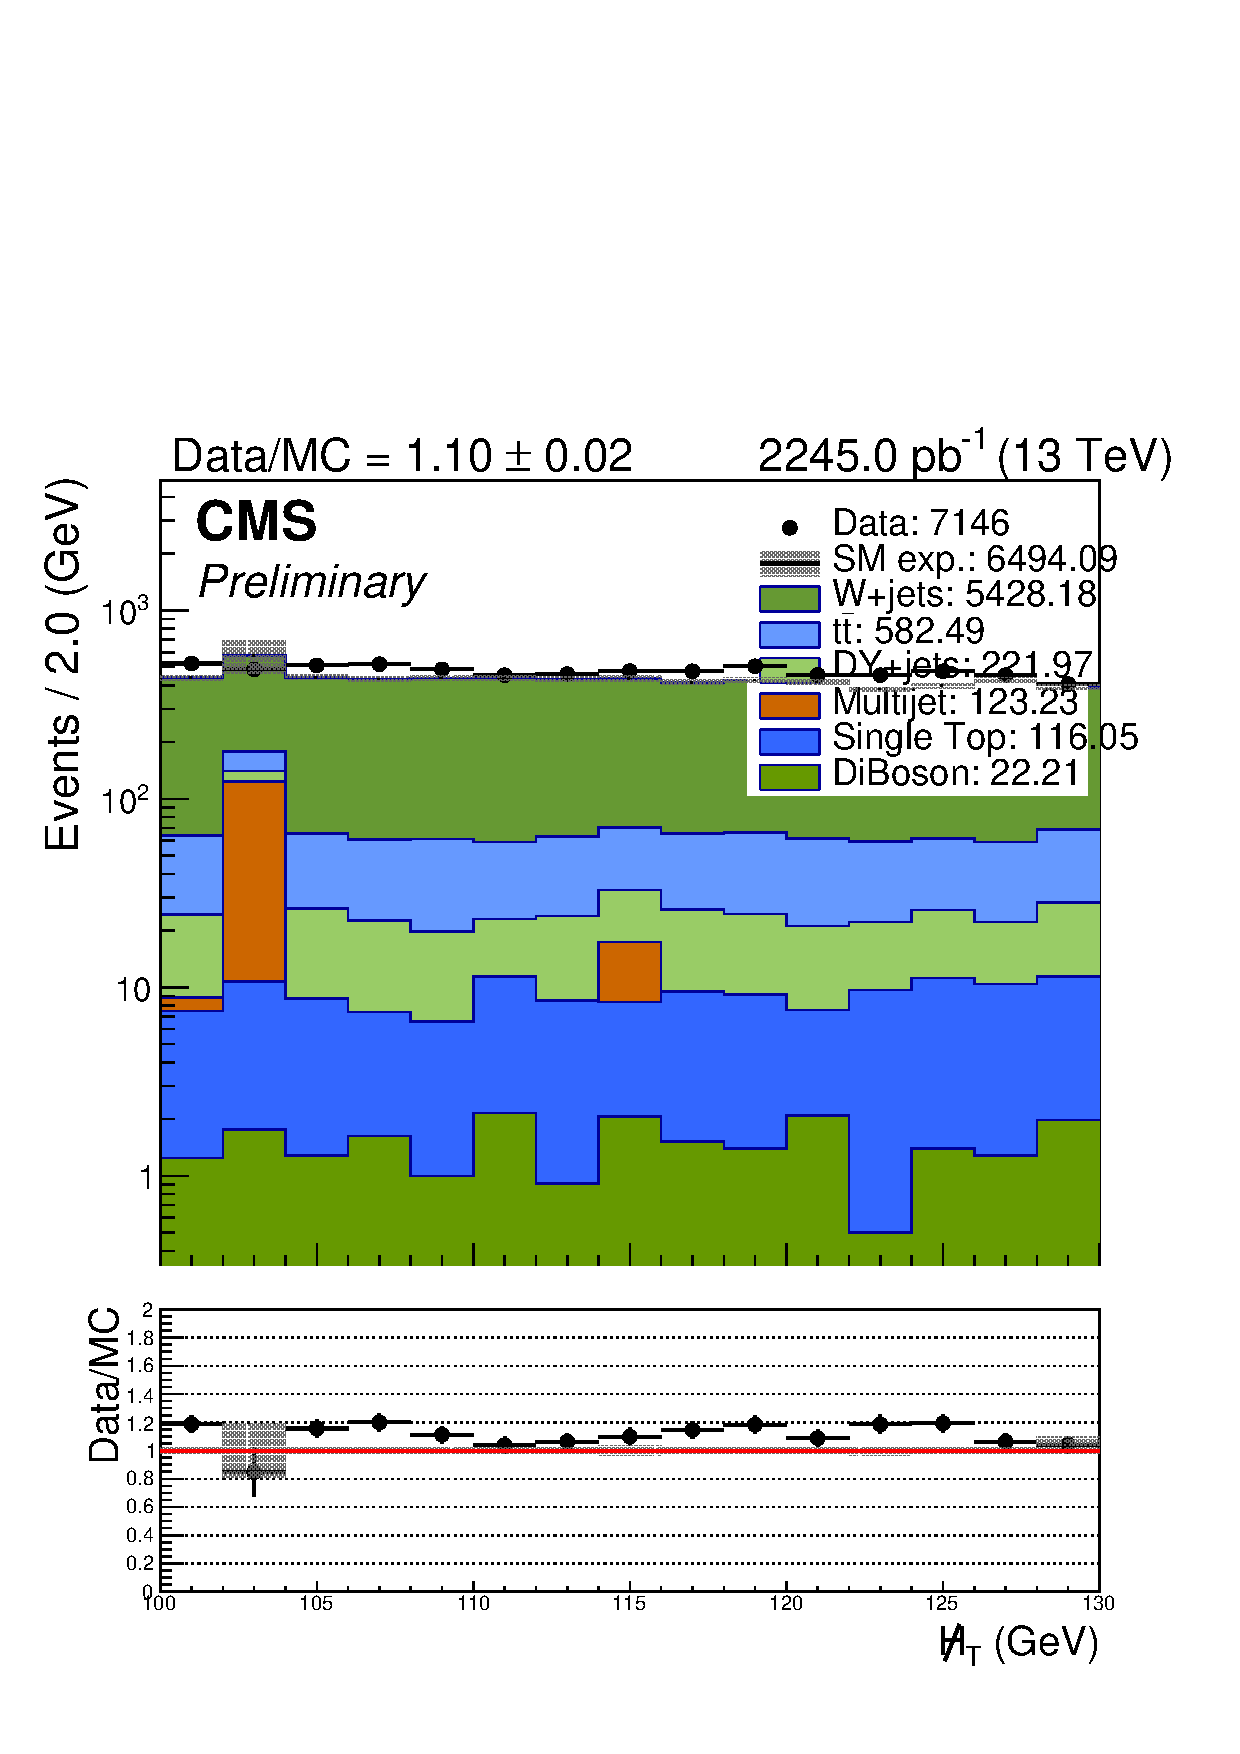
\includegraphics[width=0.45\textwidth]{figures/sidebandCorr/mhtSideband_NMinusOne_MHT_WJets}
  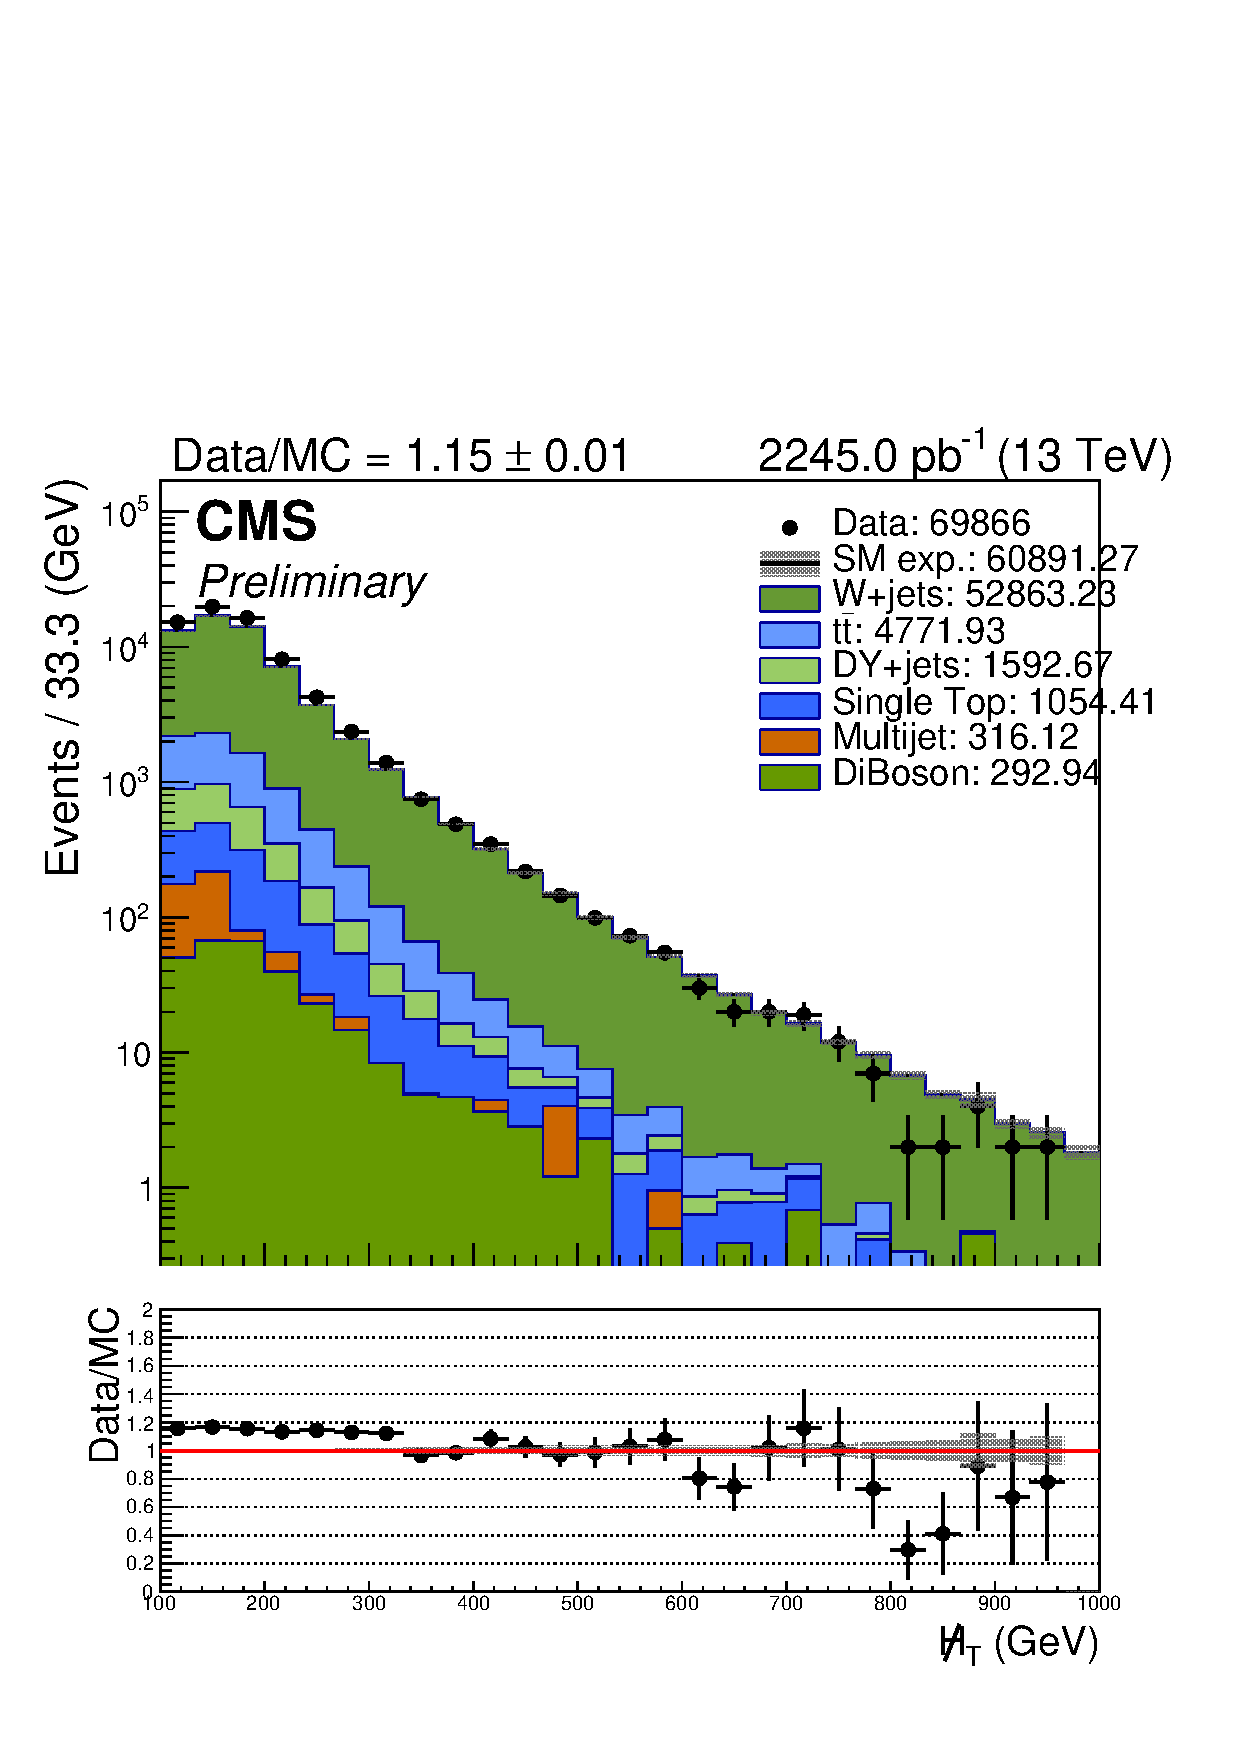
\includegraphics[width=0.45\textwidth]{figures/sidebandCorr/mht_NMinusOne_MHT_WJets}
  \caption{The \mht distribution in the \wj-enriched sample in the \mj control region in data compared with MC expectations. 
     The \mht sideband used to derive the correction for the \wj process is shown on the left plot, while the full range is shown on the right.}
  \label{fig:wjets_MHTsideband}
\end{figure}

\begin{figure}[!h]
  \centering
  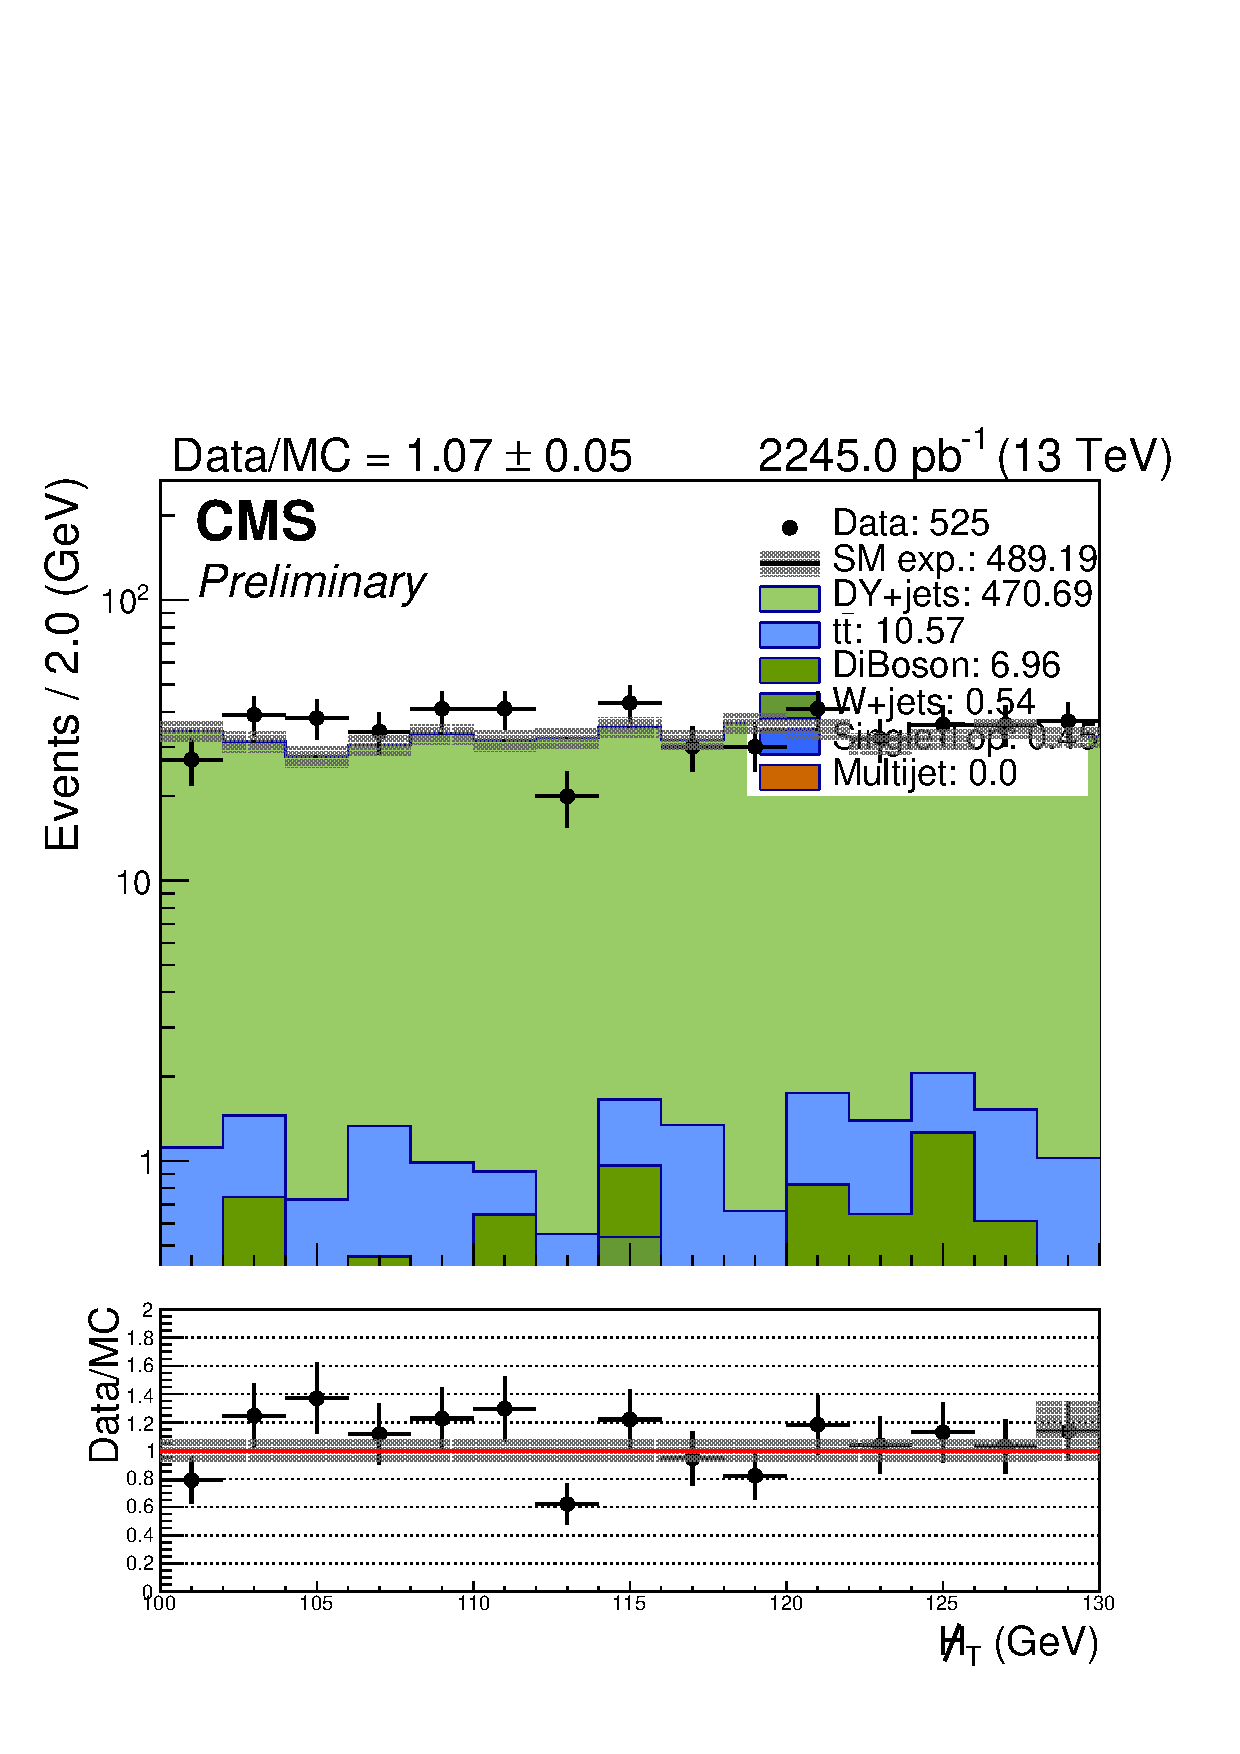
\includegraphics[width=0.45\textwidth]{figures/sidebandCorr/mhtSideband_NMinusOne_MHT_DYJetsToLL}
  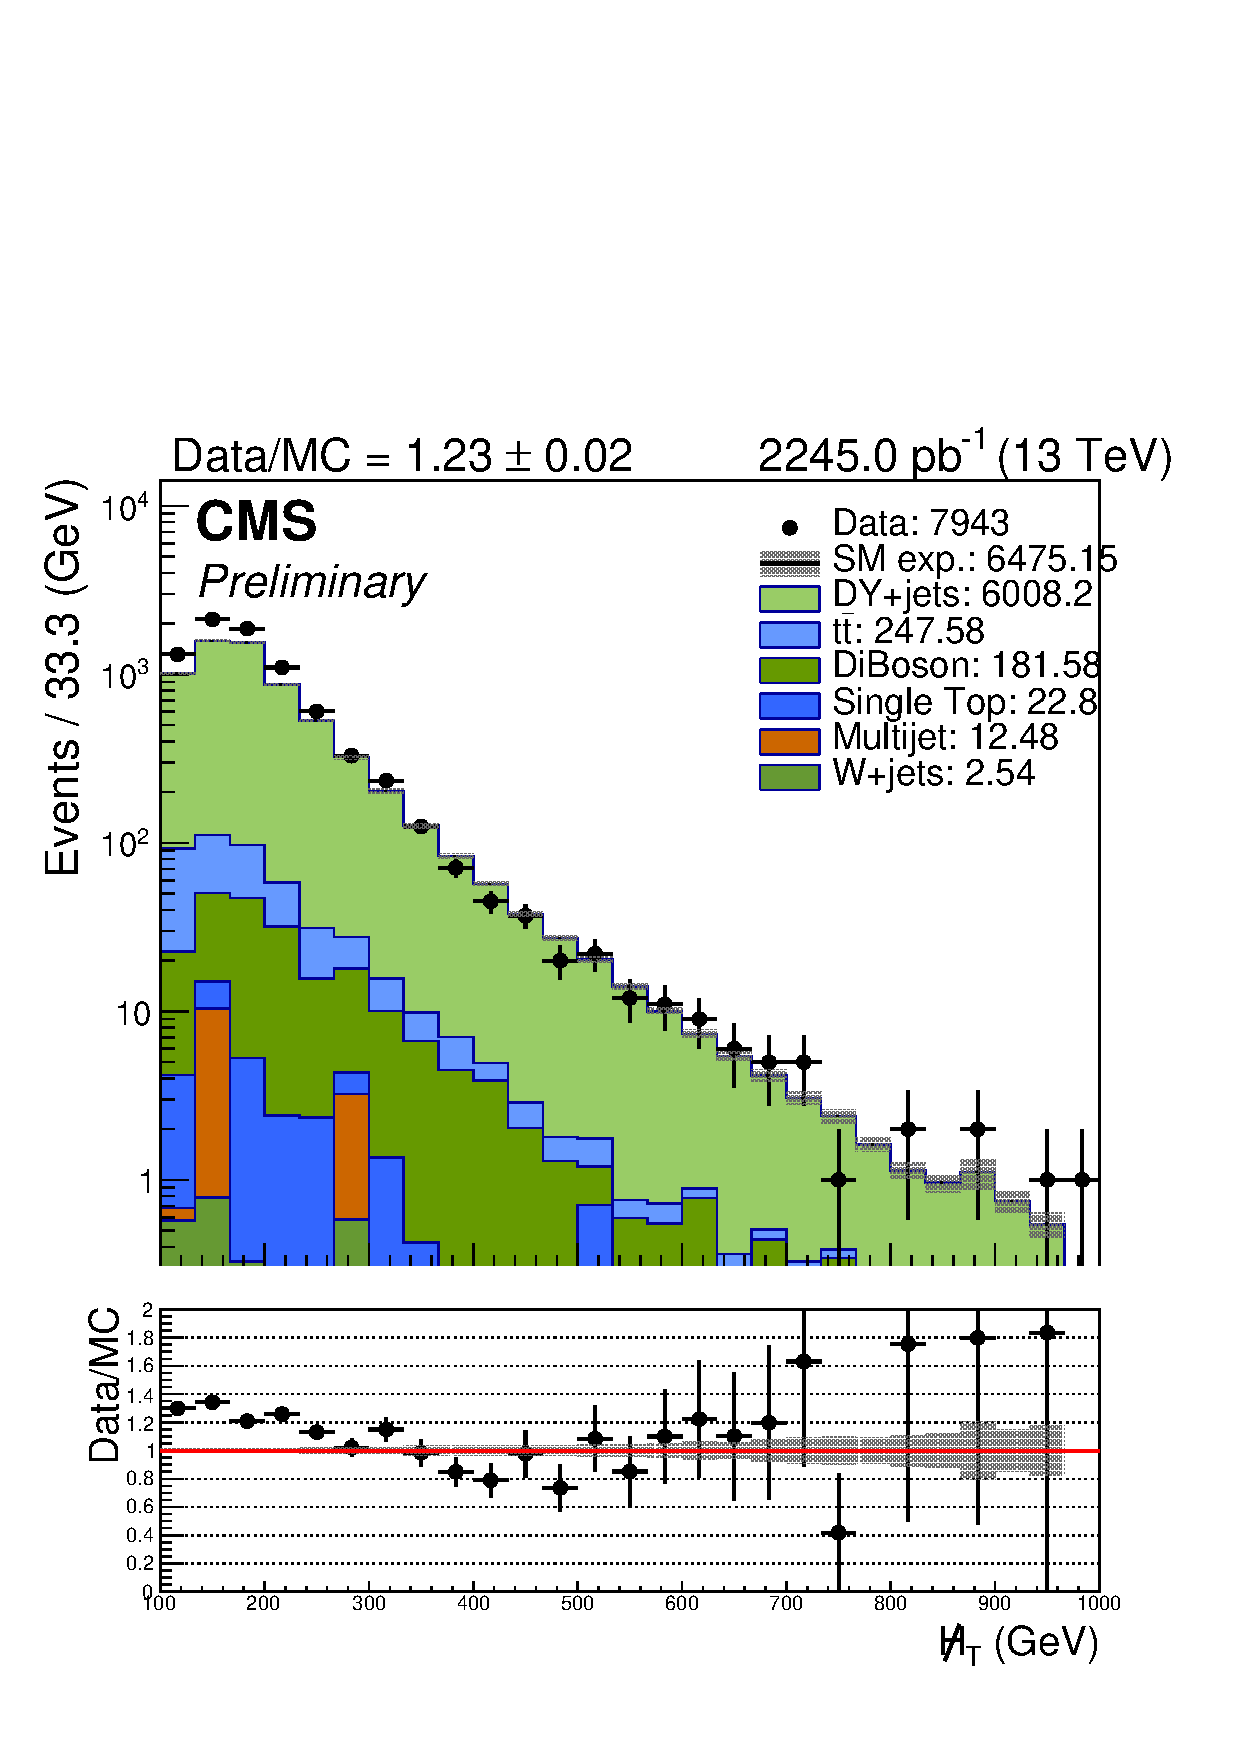
\includegraphics[width=0.45\textwidth]{figures/sidebandCorr/mht_NMinusOne_MHT_DYJetsToLL}
  \caption{The \mht distribution in the \zj-enriched sample in the \mmj control region in data compared with MC expectations. 
     The \mht sideband used to derive the correction for the \zj process is shown on the left plot, while the full range is shown on the right.}
  \label{fig:zjets_MHTsideband}
\end{figure}

\begin{figure}[!h]
  \centering
  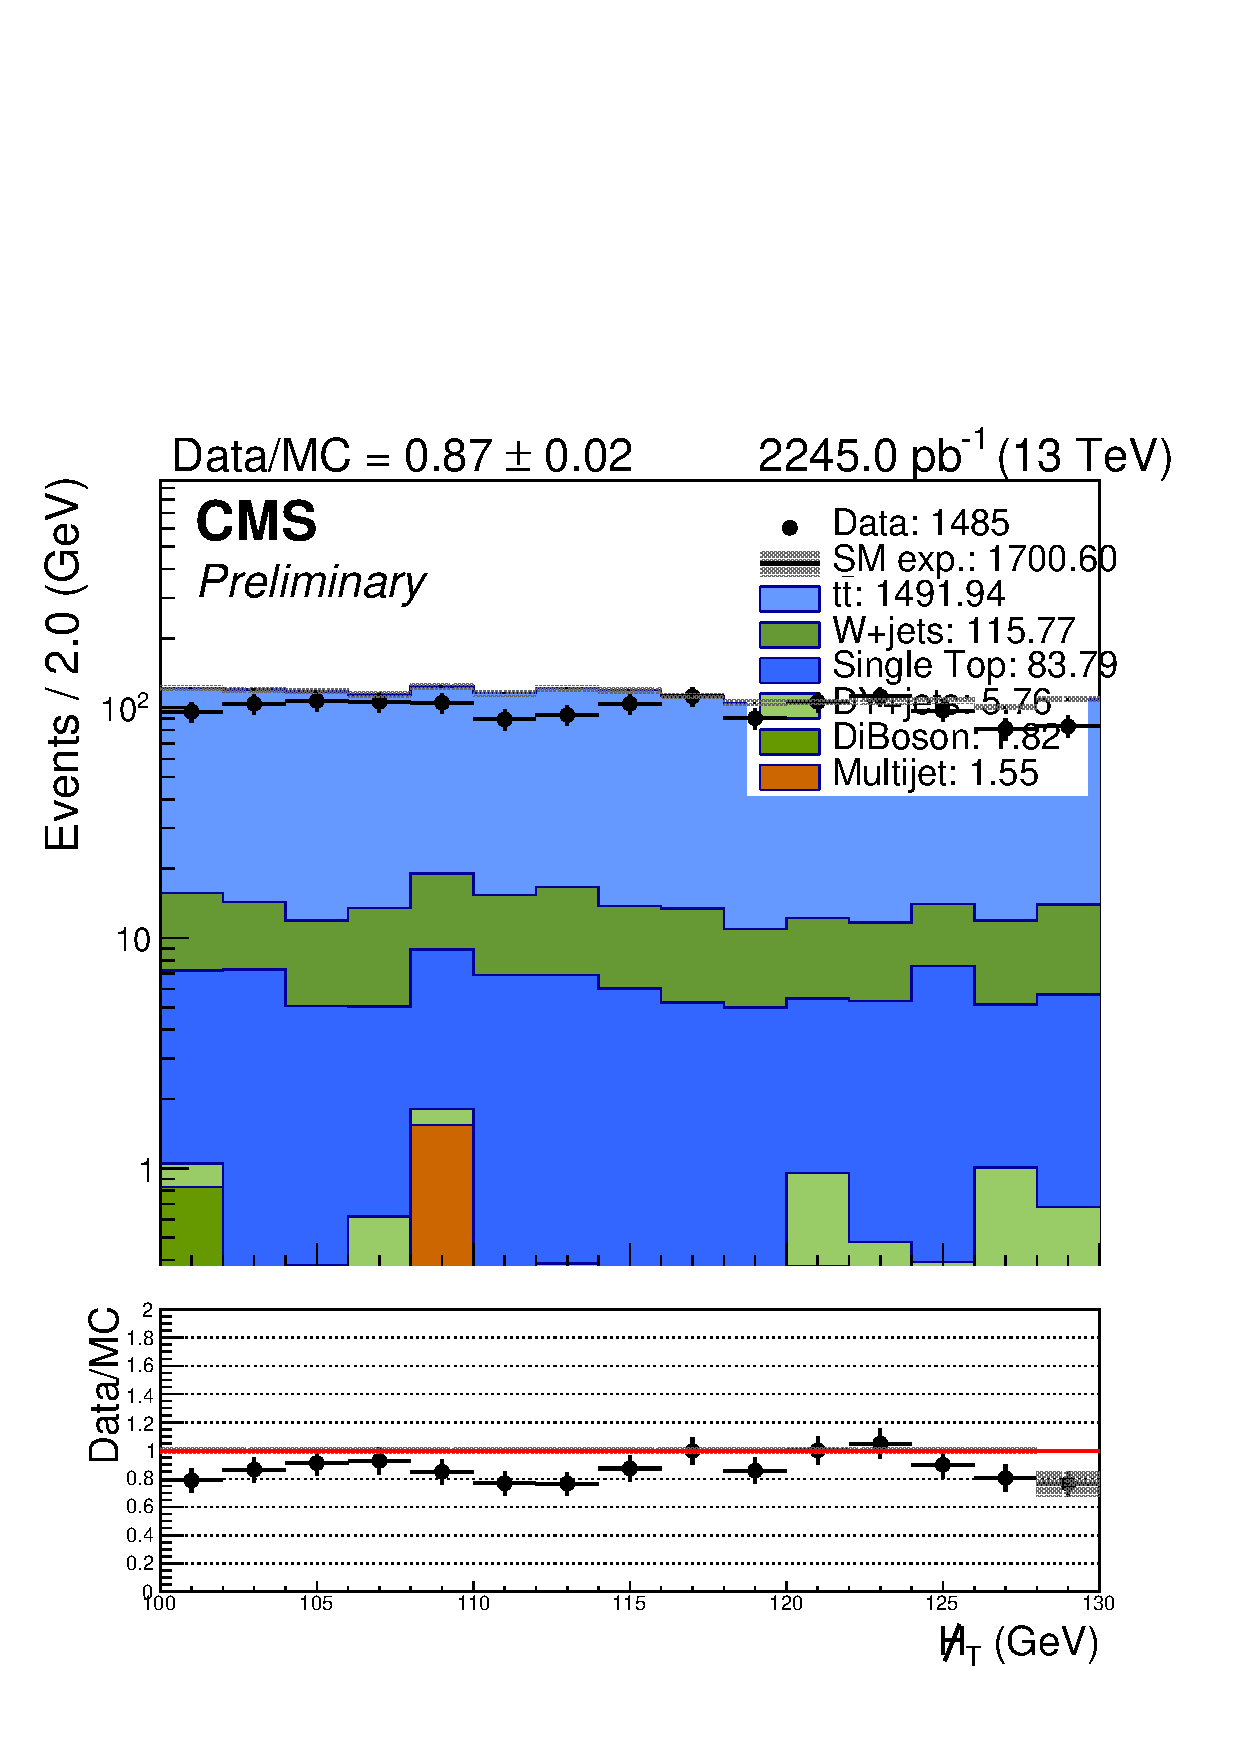
\includegraphics[width=0.45\textwidth]{figures/sidebandCorr/mhtSideband_NMinusOne_MHT_TTJets}
  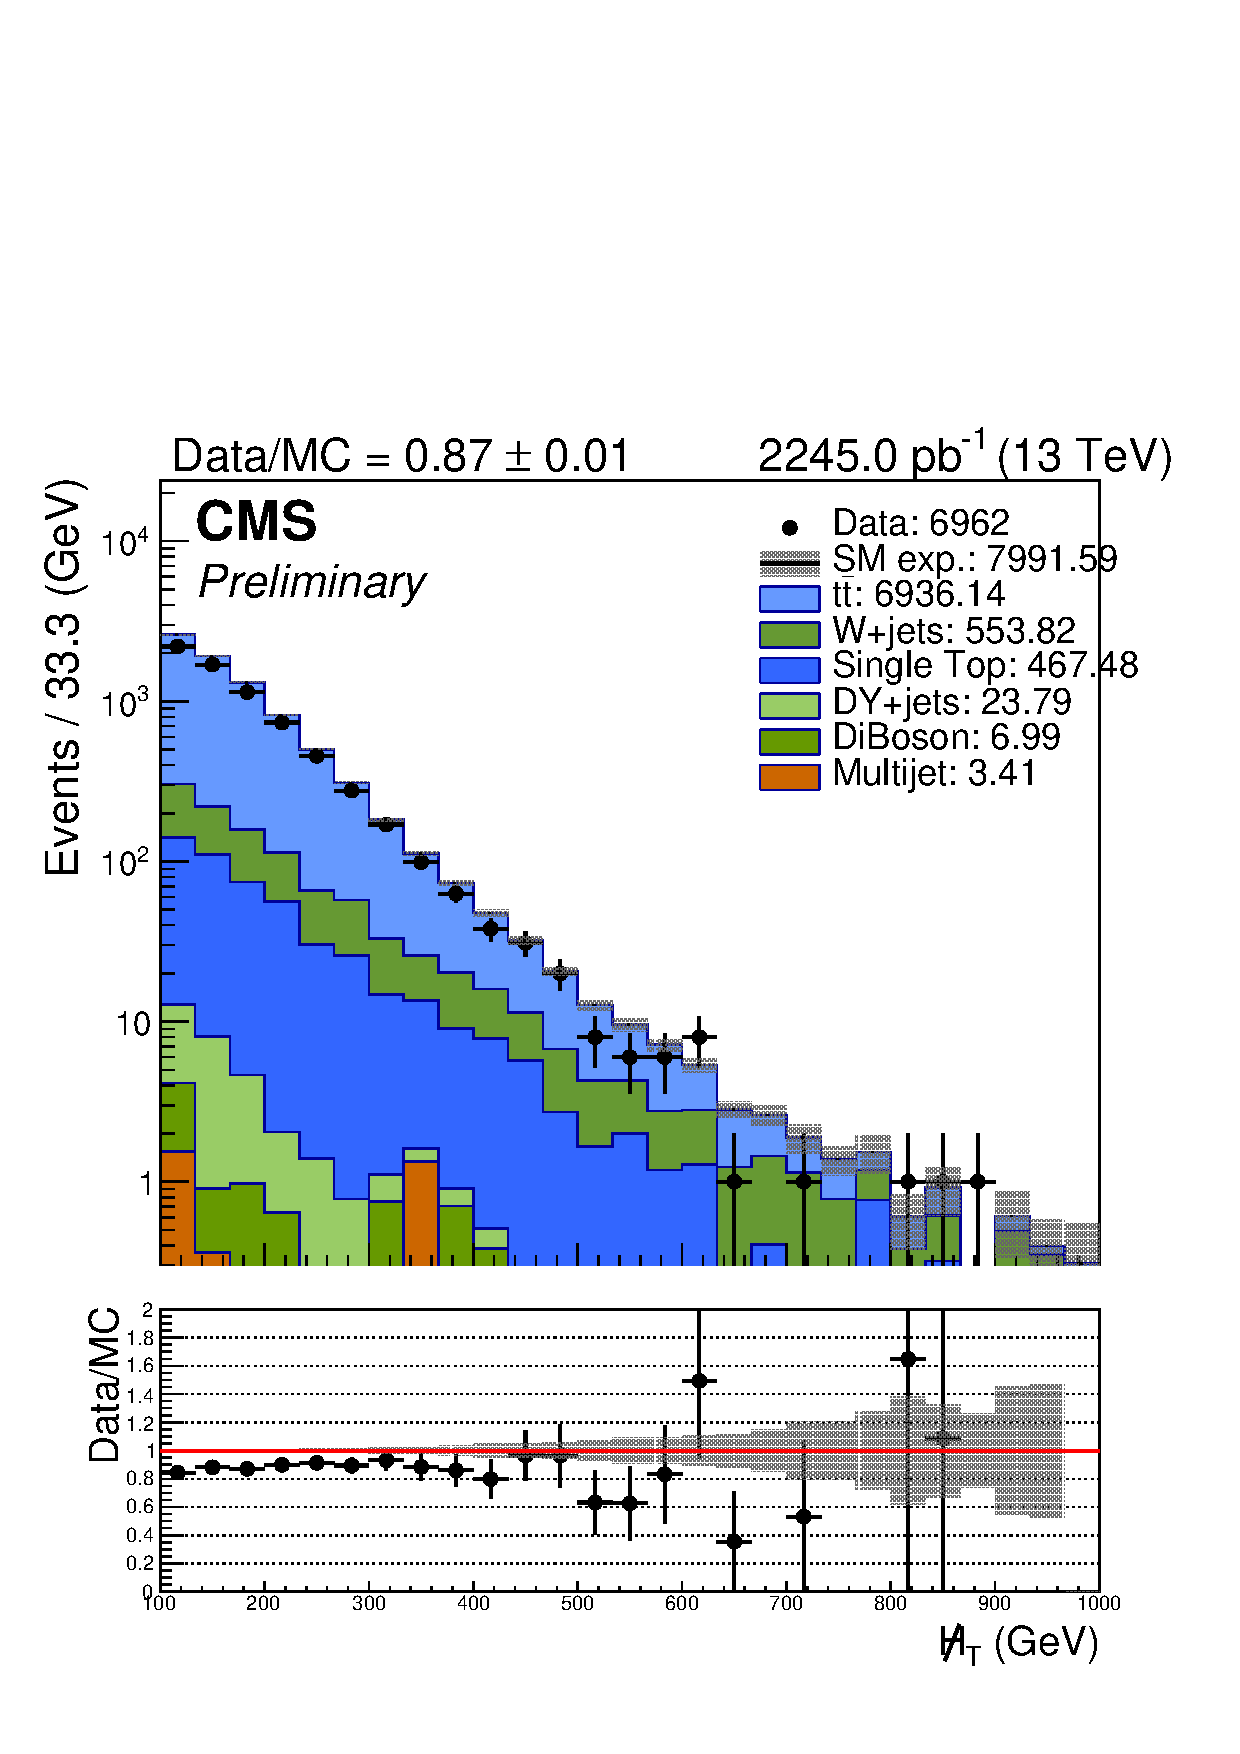
\includegraphics[width=0.45\textwidth]{figures/sidebandCorr/mht_NMinusOne_MHT_TTJets}
  \caption{The \mht distribution in the \ttbar-enriched sample in the \mj control region in data compared with MC expectations. 
     The \mht sideband used to derive the correction for the \ttbar process is shown on the left plot, while the full range is shown on the right.}
  \label{fig:ttjets_MHTsideband}
\end{figure}


\begin{table}[!h]
  \scriptsize
  \centering
  \topcaption{Cross section corrections for SM backgrounds derived with sidebands in data. Uncertainty is statistical-only.}
  \label{tab:sbCorrs}
  \begin{tabular}
    {cllc}
    \hline\hline
    \textbf{Process} & \textbf{Sideband} & \textbf{Selection} & \textbf{Corrrection} \\
    \hline
    \gj & $0.50 < \alphat < 0.52(0.53)$ & \gj & $1.25 \pm 0.10$ \\
    \wj & $100 < \mht < 130 \, \mathrm{GeV}$ & \mj, $\nj \leq 3$, $\nb = 0$ & $1.12 \pm 0.03$ \\
    \zj & $100 < \mht < 130 \, \mathrm{GeV}$ & \mmj, $\nb = 0$ & $1.08 \pm 0.05$ \\
    \ttbar + jets & $100 < \mht < 130 \, \mathrm{GeV}$ & \mj, $\nj \geq 2$, $\nb \geq 2$ & $0.86 \pm 0.03$ \\
    \hline \hline
  \end{tabular}
\end{table}



%% In Fig.~\ref{fig:sfVsHt}, the correction factor derived from the \mhtmet sideband is extracted in coarse bins in \scalht for the 3 processes. 
%% Since the analysis is sensitive to relative corrections rather than absolute ones, the 3 ratios of correction factors 
%% are showed in Fig.~\ref{fig:double_ratios}. They are compatible with flat within the statistical uncertainties. 
%% Therefore any \scalht dependence approximately cancels out in the ratio of transfer factors, thus any correction would have a negligible impact. \\
%% For an inclusive correction, as stated previously, a better understanding of detector effects is required and thus this study is postponed. 

%% \begin{figure}[!h]
%%  \centering
%%  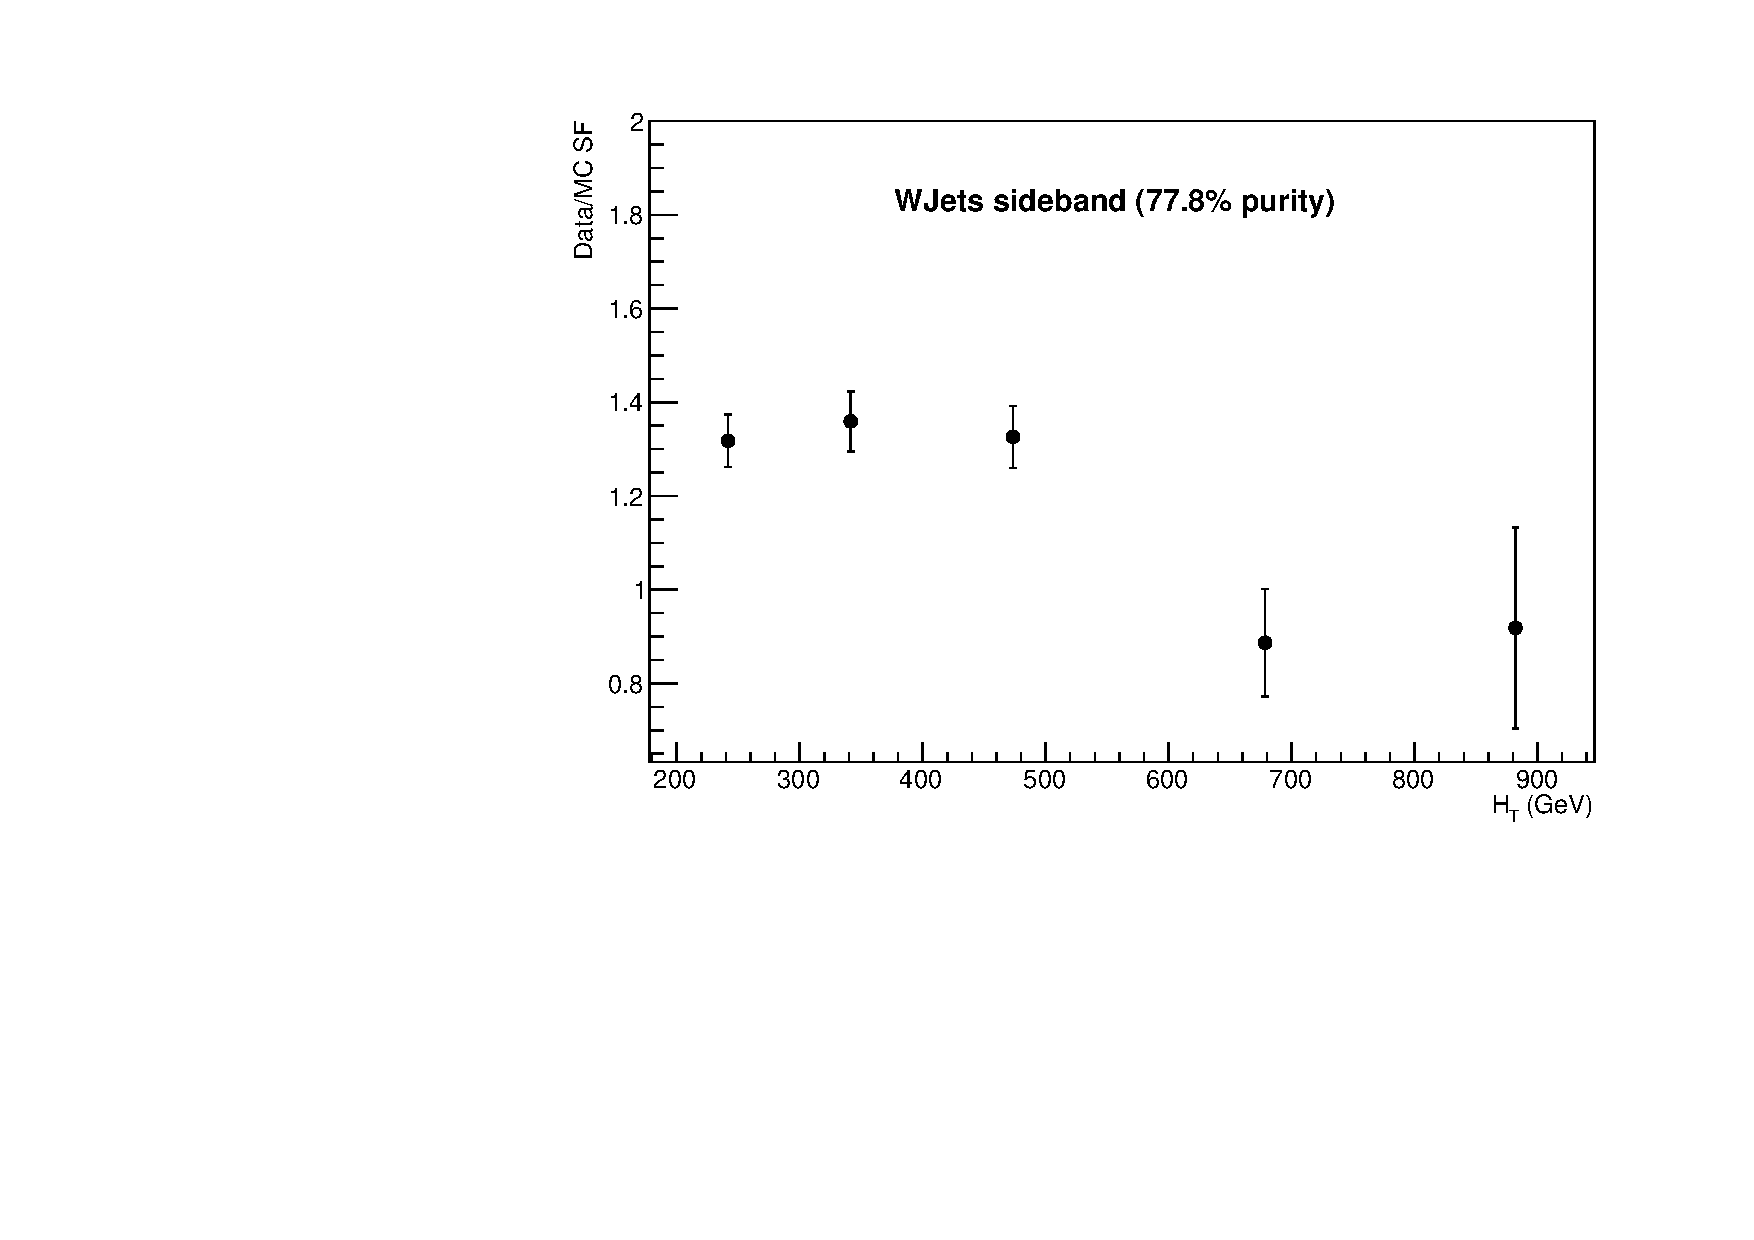
\includegraphics[width=0.31\textwidth]{figures/sidebandCorr/SFvsHT_MHTOverMET_WJets}
%%  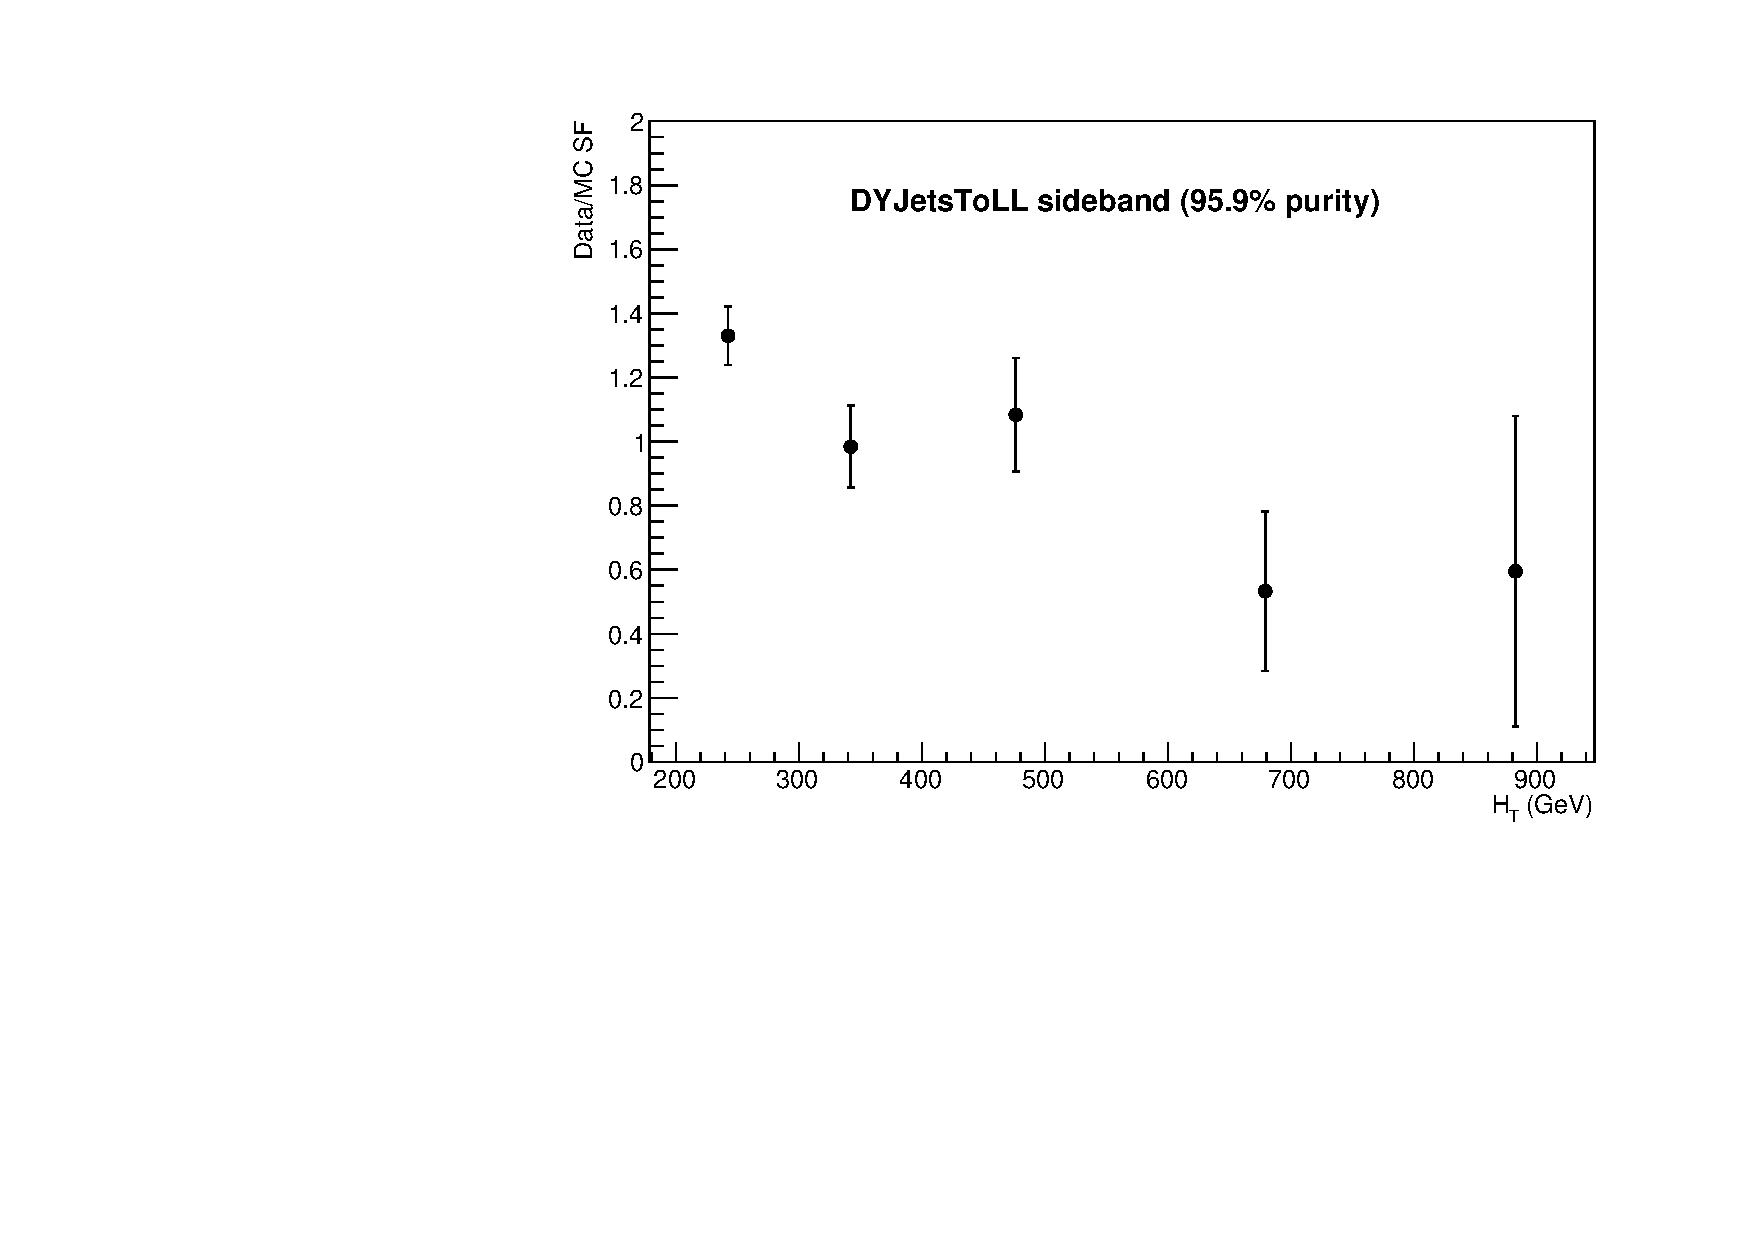
\includegraphics[width=0.31\textwidth]{figures/sidebandCorr/SFvsHT_MHTOverMET_DYJetsToLL}
%%  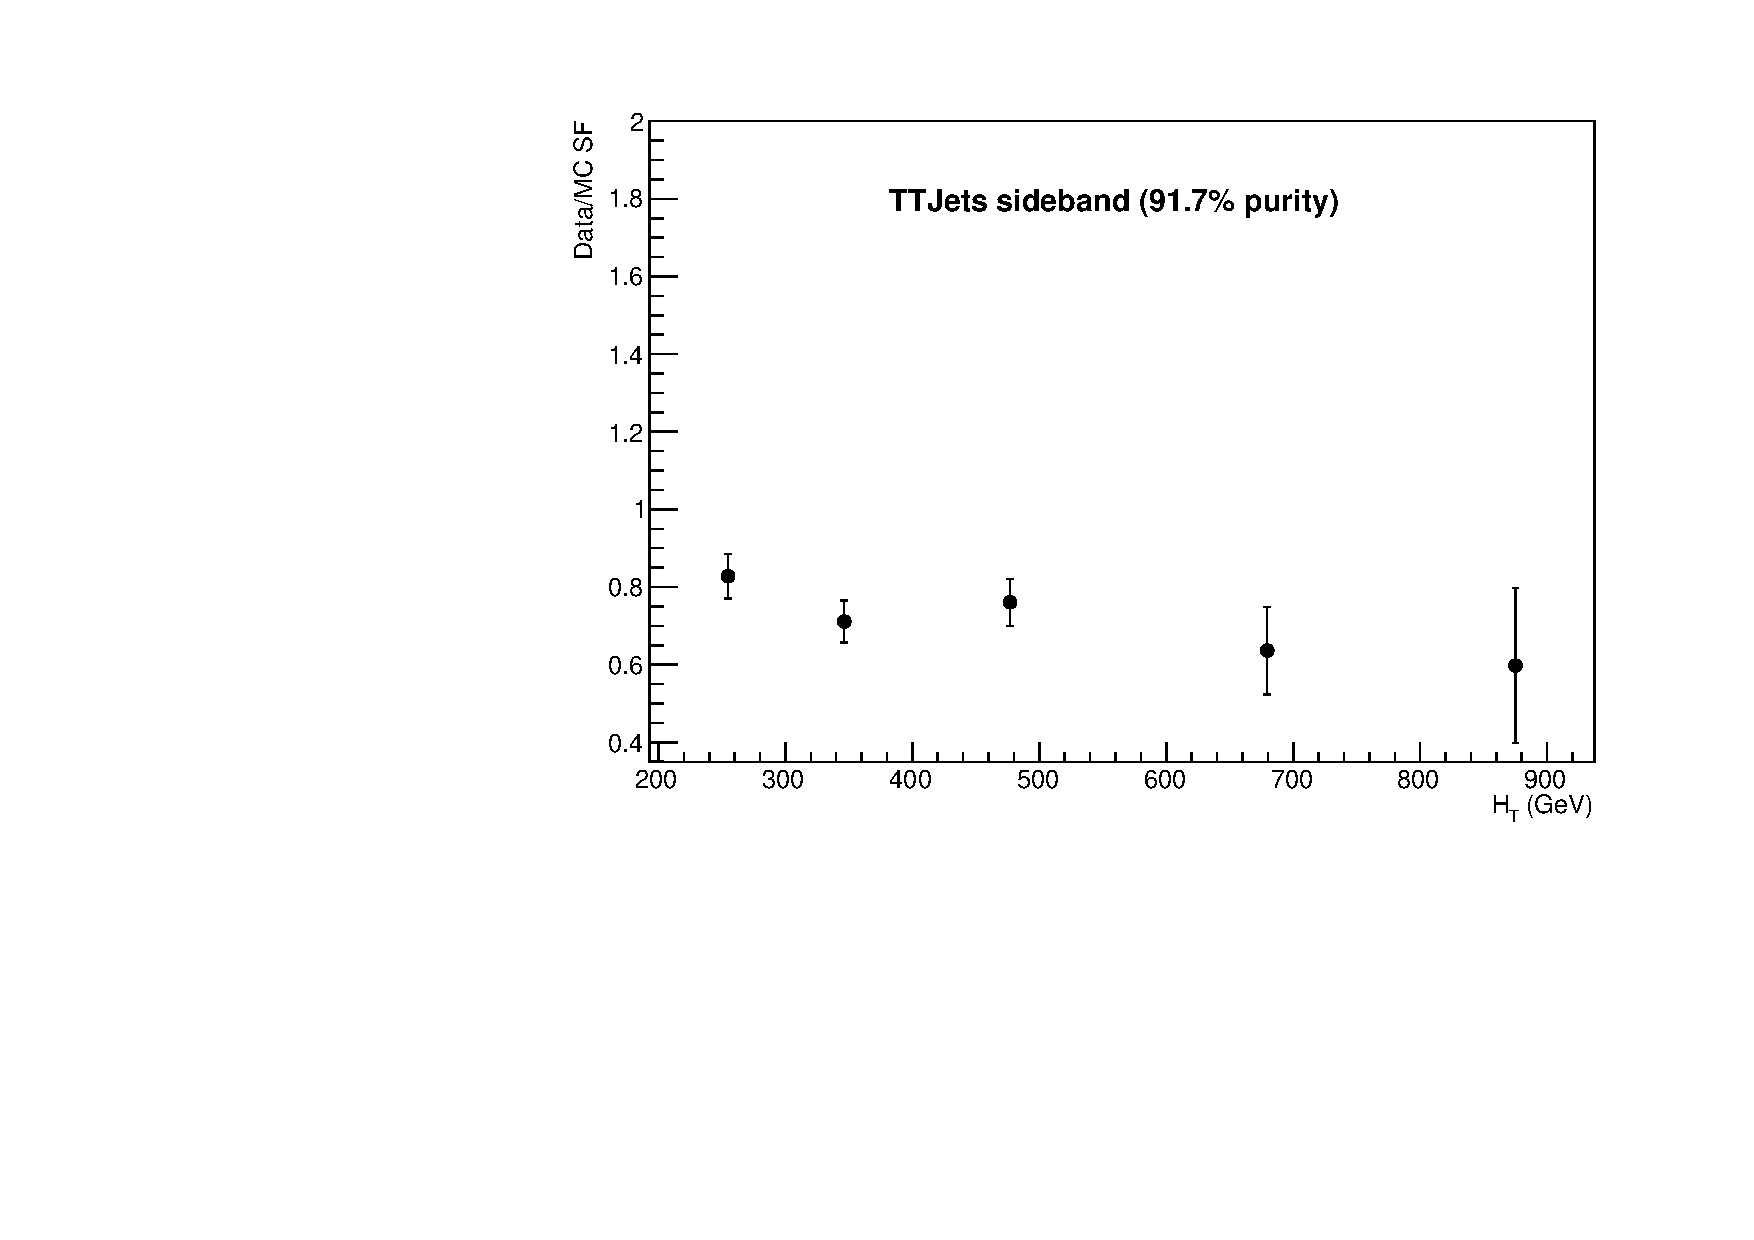
\includegraphics[width=0.31\textwidth]{figures/sidebandCorr/SFvsHT_MHTOverMET_TTJets}
%%  \caption{The correction factor as a function of \scalht for the \wj (left), \zj (center) and \ttj (right) selection.}
%%  \label{fig:sfVsHt}
%% \end{figure}

%% \begin{figure}[!h]
%%  \centering
%%  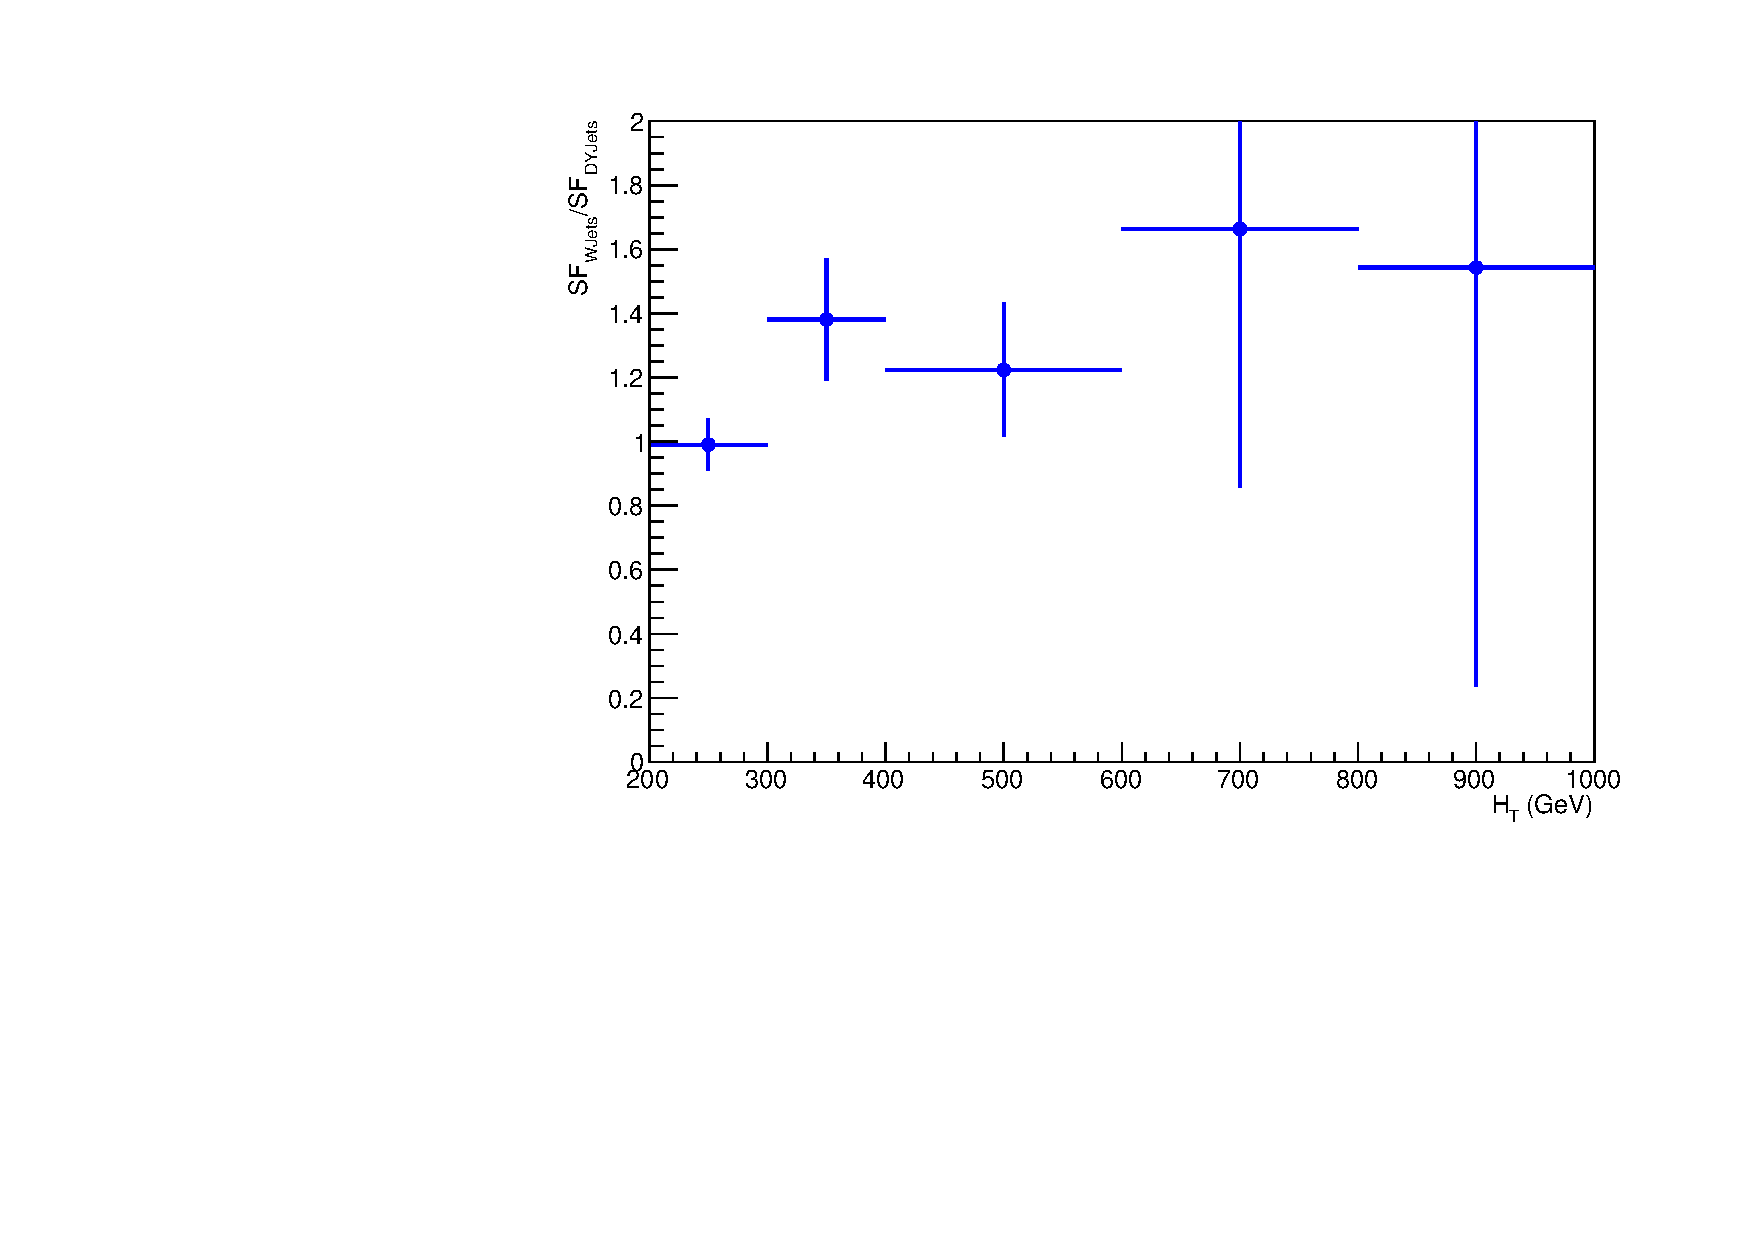
\includegraphics[width=0.31\textwidth]{figures/sidebandCorr/SFDR_w_z}
%%  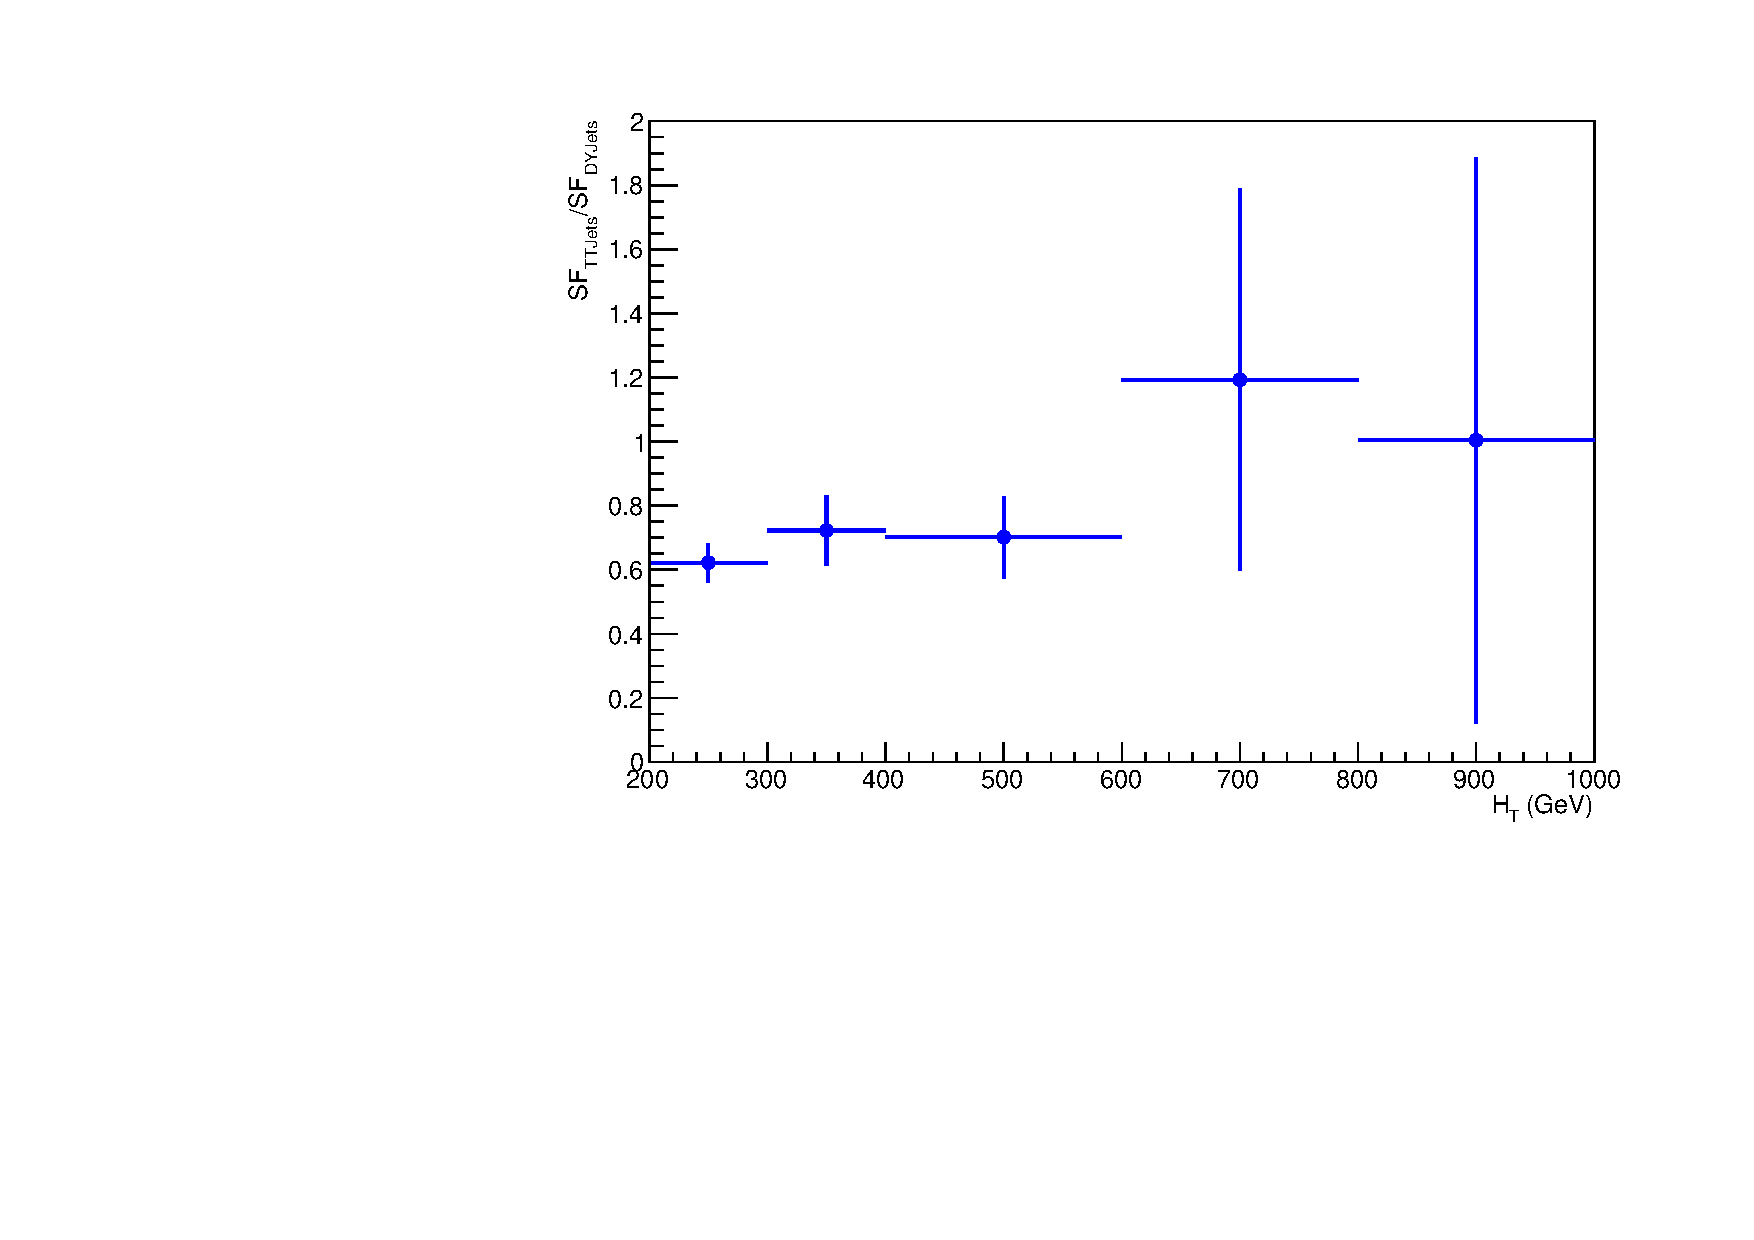
\includegraphics[width=0.31\textwidth]{figures/sidebandCorr/SFDR_tt_z}
%%  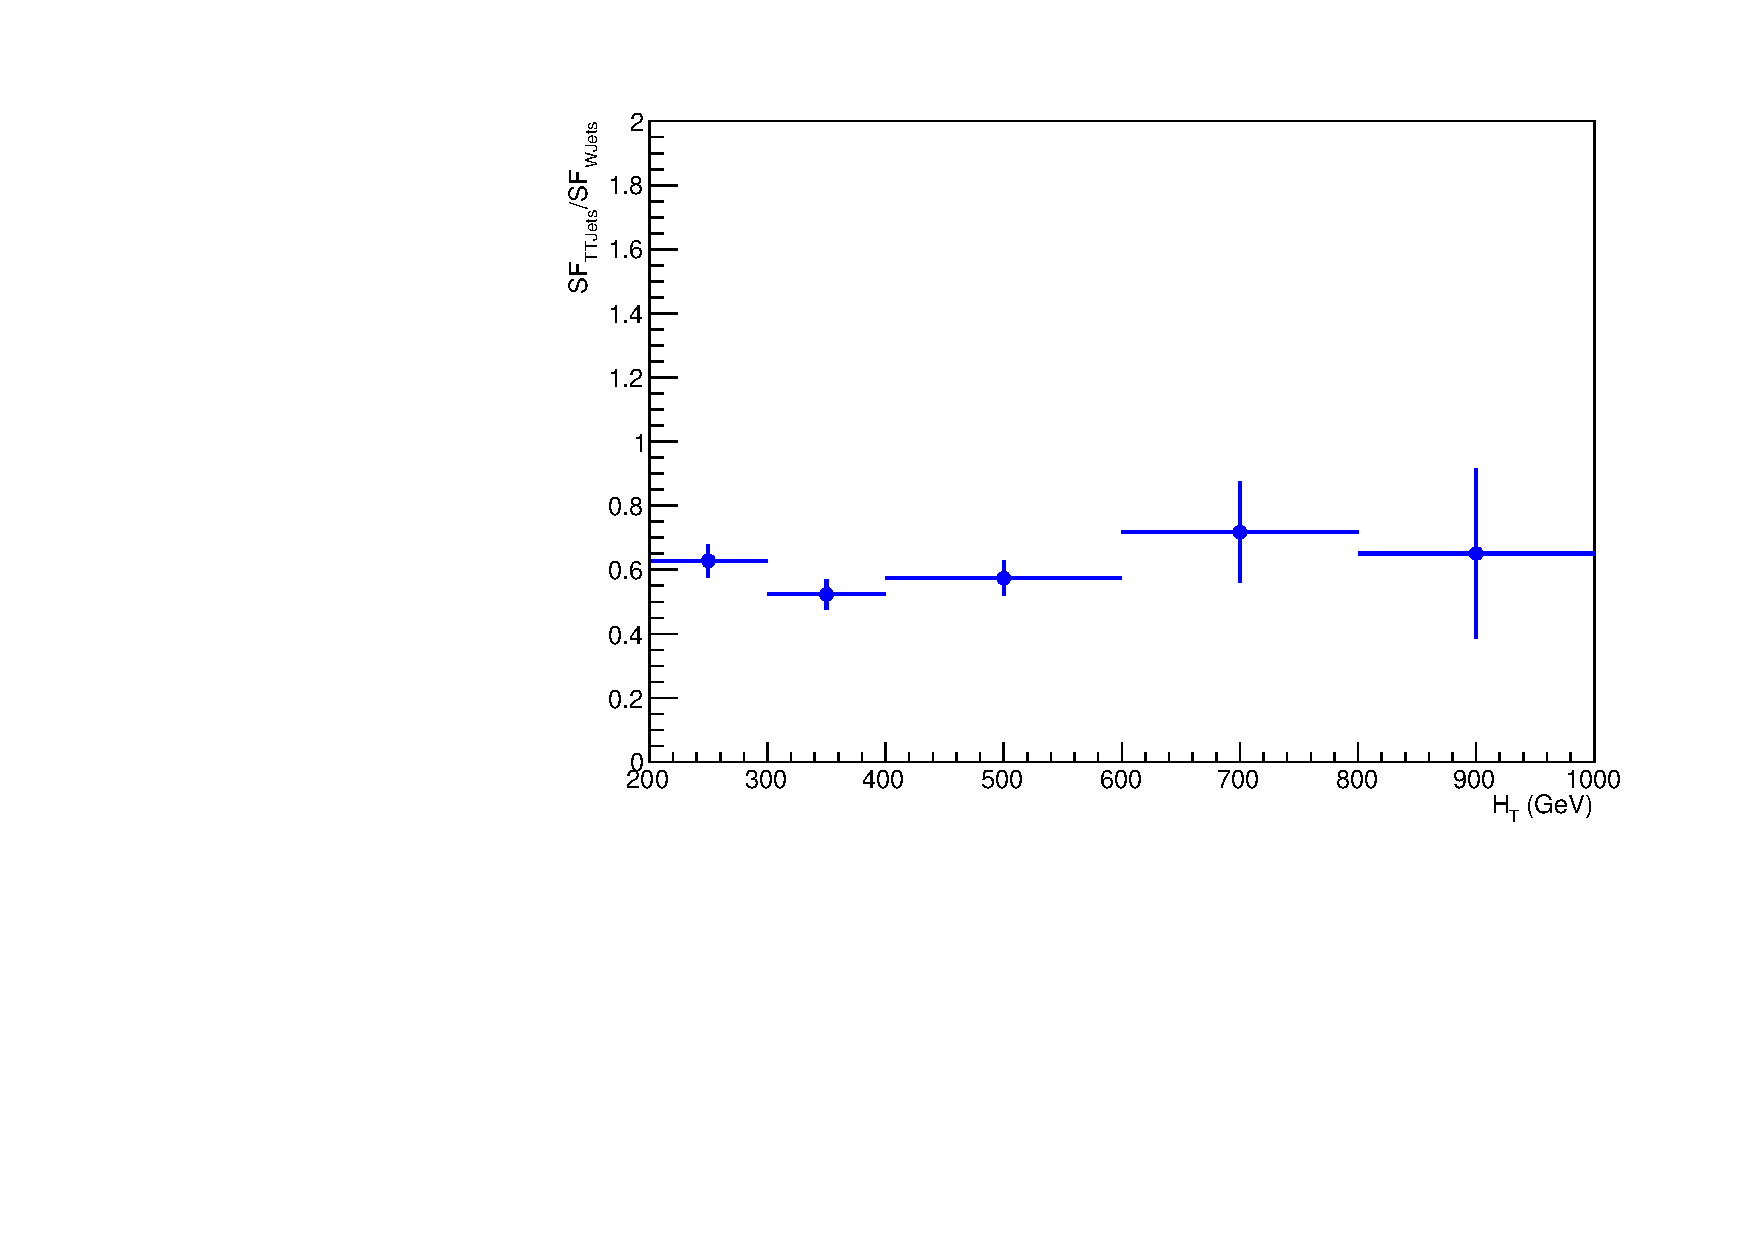
\includegraphics[width=0.31\textwidth]{figures/sidebandCorr/SFDR_tt_w}
%%  \caption{The ratio of correction factors as a function of \scalht: \wj/\zj (left), \ttj/\zj (center) and \ttj/\wj (right).}
%%  \label{fig:double_ratios}
%% \end{figure}

